\documentclass[../defence.tex]{subfiles}

\begin{document}
  \begin{frame}{Bad pore opening}
    \begin{columns}[onlytextwidth, T]
      \column{\dimexpr\linewidth / 21 * 10}
        \tikzsetnextfilename{294}
        \begin{tikzpicture}[scale=0.5, transform shape]
            \def\PrelMin{.86}
    				\def\PrelMax{1}
    				\def\TransMin{1e-8}
    				\def\TransMax{1}
    				\def\LfMin{0}
    				\def\LfMax{2}
            %
            \begin{axis}[
              /tikz/line join=bevel,
              grid,
    					axis y line*=left,
              legend style={at={(0,.5)}, legend columns=1, anchor=north west},
              every axis plot,
    					axis y line*=left,
    					line width = 1pt,
    					xmin = \PrelMin, xmax = \PrelMax,
    					ymin = \LfMin, ymax = \LfMax,
    					xlabel = {Relative pressure $P_\mathrm{rel}$},
    					ylabel = {Liquid fraction $LF$},
    					ytick = {0,0.25,0.50,0.75,1},
              ]
    					% Add plots
              \addplot +[no markers, raw gnuplot, line width = 1pt,red]
              gnuplot{plot "tikz/graphs/294_bad_open_pores/PNO_OuvertSol.qgra.text" index 0;};
              \addlegendentry{Closed pores}
              \addplot +[no markers, raw gnuplot, line width = 1pt,red!50]
              gnuplot{plot "tikz/graphs/294_bad_open_pores/PNO_OuvertSol.qgra.text" index 1;};
              %\addlegendentry{$LF_\mathrm{evap}^\mathrm{294cp}$}
              \addplot +[no markers, raw gnuplot, line width = 1pt,blue]
              gnuplot{plot "tikz/graphs/294_bad_open_pores/PO.qgra.text" index 0;};
              %\addlegendentry{$LF_\mathrm{cond}^\mathrm{294op}$}
              \addplot +[no markers, raw gnuplot, line width = 1pt,blue!50]
              gnuplot{plot "tikz/graphs/294_bad_open_pores/PO.qgra.text" index 1;};
              %\addlegendentry{$LF_\mathrm{evap}^\mathrm{294op}$}
            \end{axis}
            %
            \begin{axis}[
              /tikz/line join=bevel,
              ymode=log,
              axis y line*=right, ylabel near ticks, yticklabel pos=right,
              line width = 1pt,
              xmin = \PrelMin, xmax = \PrelMax,
              ymin = \TransMin, ymax = \TransMax,
              ylabel = {Transmission $T$},
              ytick = {1e-1,1e-2,1e-3,1e-4},
              ymajorgrids=true,
              legend style={at={(0,0.5)}, legend columns=1, anchor=south west},
              ]
    					% Add plots
              \addplot +[no markers, raw gnuplot, line width = 1pt,red]
              gnuplot{plot "tikz/graphs/294_bad_open_pores/PNO_OuvertSol.qgra.text" using ($1):($2*0.45) index 2;};
              \addplot +[no markers, raw gnuplot, line width =1pt,red!50]
              gnuplot{plot "tikz/graphs/294_bad_open_pores/PNO_OuvertSol.qgra.text" using ($1):($2*0.45) index 3;};
              %\addlegendentry{$T_\mathrm{evap}^\mathrm{294cp}$}
              \addplot +[no markers, raw gnuplot, line width = 1pt,blue]
              gnuplot{plot "tikz/graphs/294_bad_open_pores/PO.qgra.text" using ($1):($2*0.45) index 2;};
              \addlegendentry{Bad open pores}
              \addplot +[no markers, raw gnuplot, line width =1pt,blue!50]
              gnuplot{plot "tikz/graphs/294_bad_open_pores/PO.qgra.text" using ($1):($2*0.45) index 3;};
              %\addlegendentry{$T_\mathrm{evap}^\mathrm{294op}$}
            \end{axis}
        \end{tikzpicture}
        \pause
         \begin{alertblock}{Condensation branch}
           \begin{itemize}
             \item Starts at equilibrium pressure
             \item Slope more inclined than for closed pores
           \end{itemize}
         \end{alertblock}
         \pause

      \column{\dimexpr\linewidth / 21}
      \column{\dimexpr\linewidth / 21 * 10}
        \begin{alertblock}{Evaporation branch}
          \begin{itemize}
            \item Superimposed with closed pores
          \end{itemize}
        \end{alertblock}
        \pause

        \centering
        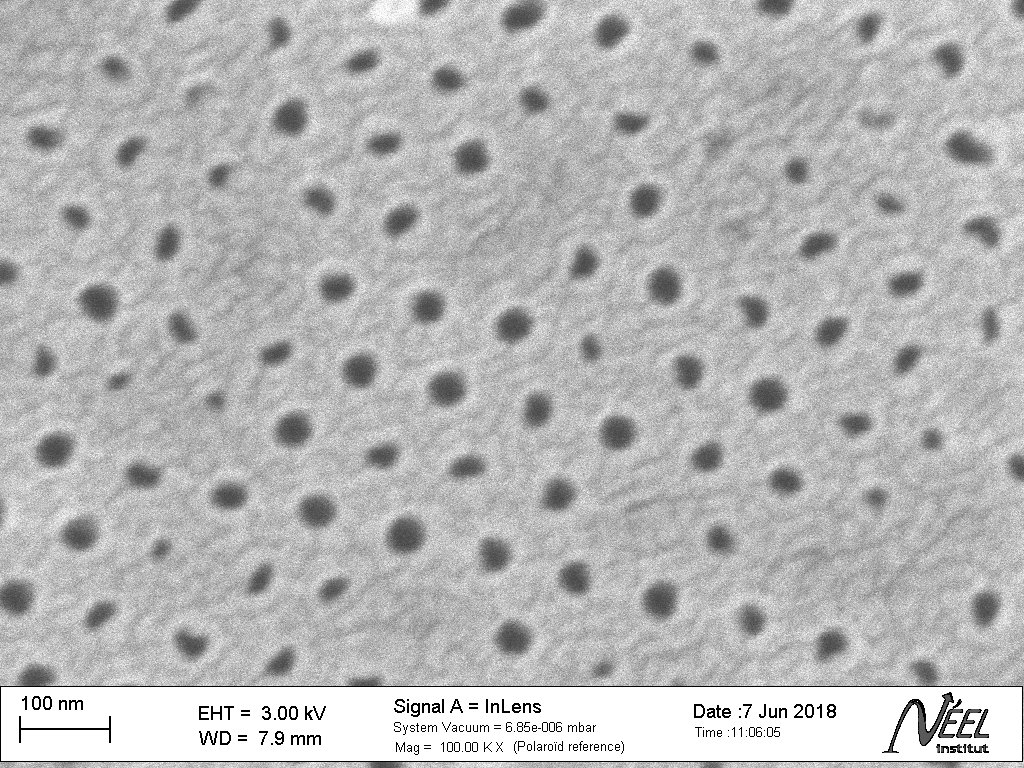
\includegraphics[width=\linewidth]{images/294_bad_open_pores.jpg}
    \end{columns}
  \end{frame}
\end{document}
